\documentclass[xcolor=dvipsnames]{beamer}
\usepackage[T1]{fontenc}
\usepackage[utf8]{inputenc}
\usepackage[english,slovak]{babel}

\usepackage{amsmath}
\usepackage{amsthm}
\usetheme{Pittsburgh}
\useoutertheme{shadow}

\usepackage{graphicx}
\usepackage{caption}
\usepackage{subcaption}

\usepackage[]{algorithm2e}
\usepackage{listings}
 \setbeamercovered{transparent}
 \usepackage{cuted}
\usepackage[export]{adjustbox}
\usepackage{mathtools}

\usepackage{lipsum}
\usepackage{verbatim}
\usepackage{transparent}
\usepackage{framed}
\usepackage{xcolor}

\usepackage{multirow}
\usepackage{colortbl}
\usepackage{lmodern}

\usepackage{movie15}
\usepackage{media9}
\usepackage{verbatim}

\usepackage{animate}


\usepackage{hyperref}

\newcommand\Wider[2][3em]{%
\makebox[\linewidth][c]{%
  \begin{minipage}{\dimexpr\textwidth+#1\relax}
  \raggedright#2
  \end{minipage}%
  }%
}






\iftrue

\usetheme{Warsaw}

\setbeamercolor{normal text}{fg=white,bg=black!90}
\setbeamercolor{structure}{fg=white}

\setbeamercolor{alerted text}{fg=red!85!black}

\setbeamercolor{item projected}{use=item,fg=black,bg=item.fg!35}

\setbeamercolor*{palette primary}{use=structure,fg=structure.fg}
\setbeamercolor*{palette secondary}{use=structure,fg=structure.fg!95!black}
\setbeamercolor*{palette tertiary}{use=structure,fg=structure.fg!90!black}
\setbeamercolor*{palette quaternary}{use=structure,fg=structure.fg!95!black,bg=black!80}

\setbeamercolor*{framesubtitle}{fg=white}

\setbeamercolor*{block title}{parent=structure,bg=black!60}
\setbeamercolor*{block body}{fg=black,bg=black!10}
\setbeamercolor*{block title alerted}{parent=alerted text,bg=black!15}
\setbeamercolor*{block title example}{parent=example text,bg=black!15}

\fi



%-------------------------------------------------------------------------------------
\title{\color{white} \bf reinforcement learning tutorial}
\author{\color{white} Michal CHOVANEC, PhD}


%\setbeamertemplate{footline}[frame number]{}
\setbeamertemplate{navigation symbols}{}


\date[EURP]{}
\begin{document}

{
    \usebackgroundtemplate
    {
        \vbox to \paperheight{\vfil\hbox to \paperwidth{\hfil

        {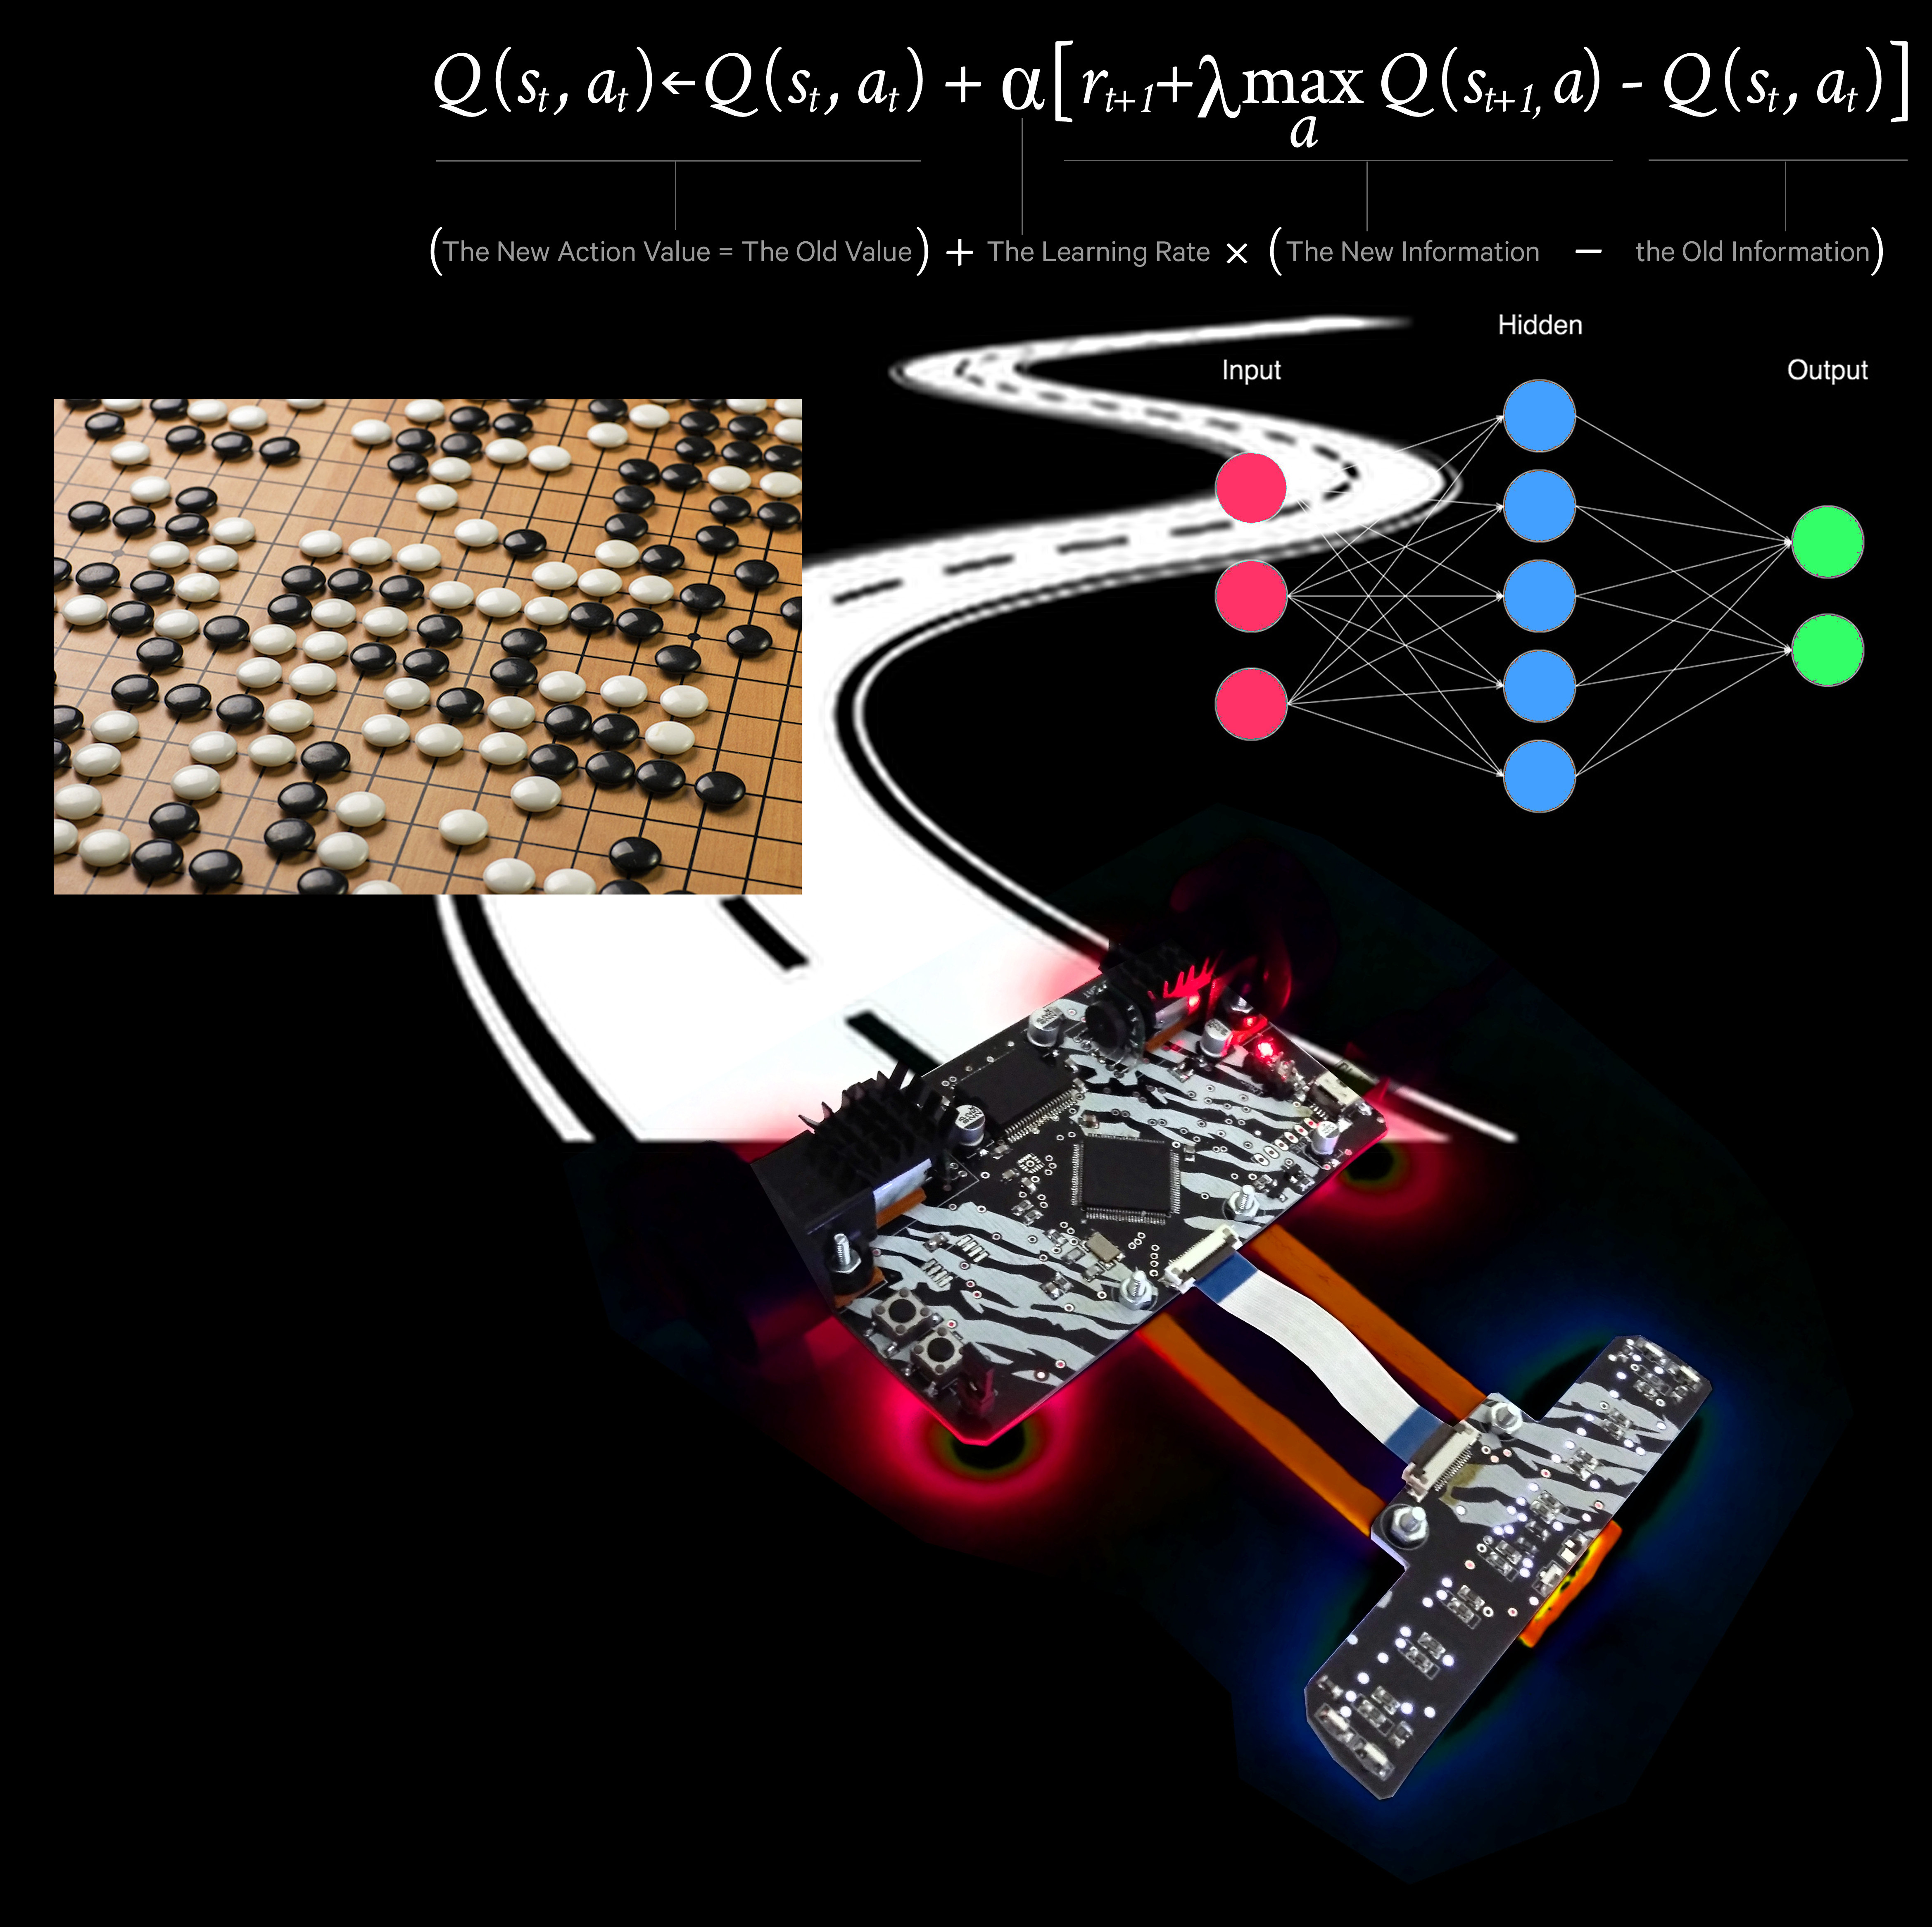
\includegraphics[width=5.05in]{../images/rl_square.jpg}}

        \hfil}\vfil}
    }



    \begin{frame}

    \centering
     \colorbox{black}
     {
        \begin{minipage}{8cm}
           {\LARGE \color{white}reinforcement learning tutorial} \\
           {\Large \color{white}- deep Q networks} \\
           {\Large \color{white}- deep deterministic policy gradient} \\
           {\LARGE \color{white} Michal CHOVANEC} \\
       \end{minipage}
     }

    \end{frame}
}



\begin{frame}{\bf reinforcement learning}

  \begin{columns}

    \begin{column}{0.5\textwidth}
      \centering{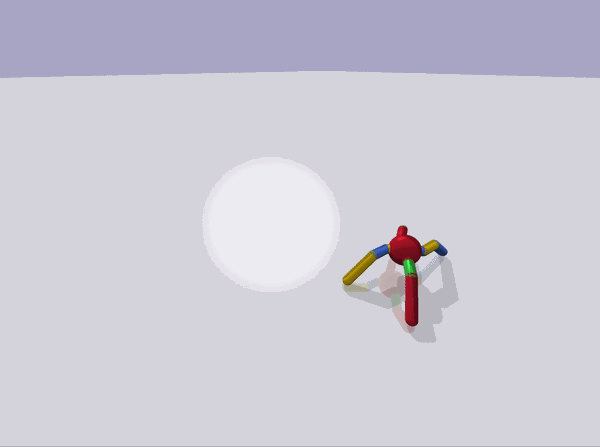
\includegraphics[scale=0.2]{../images/ant.png}}
      \centering{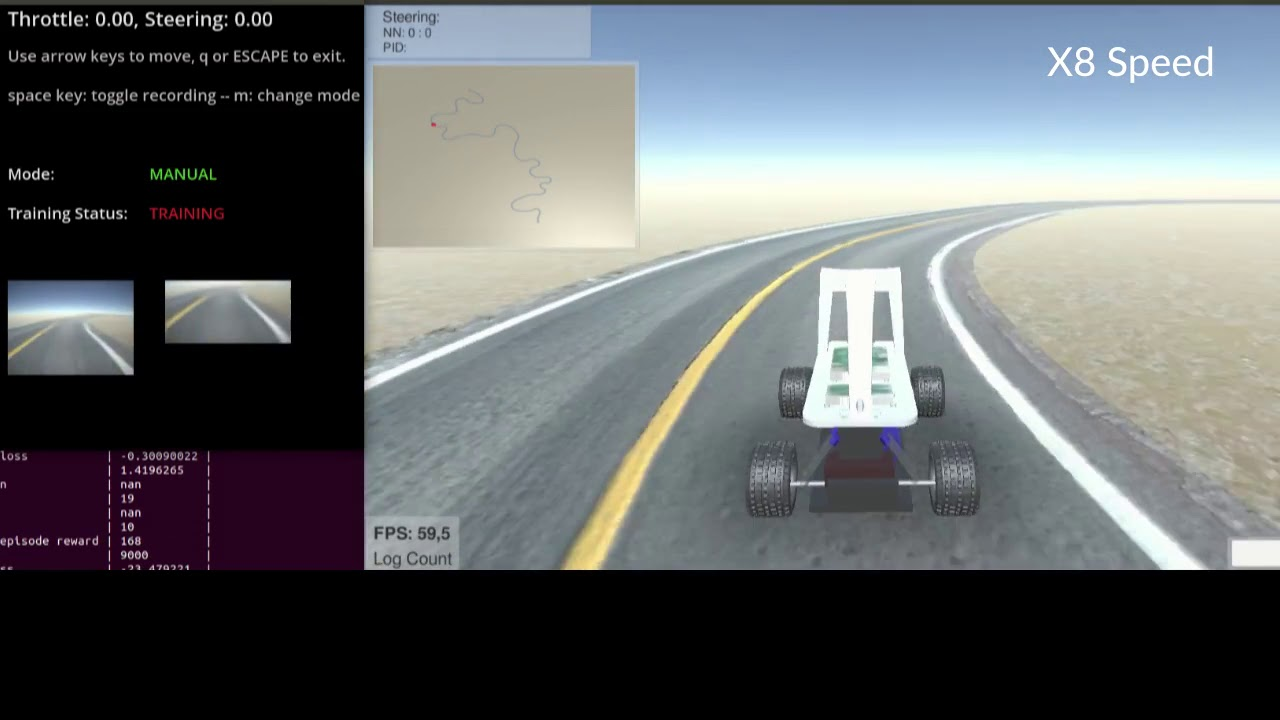
\includegraphics[scale=0.1]{../images/sac_car.jpg}}
    \end{column}

    \begin{column}{0.5\textwidth}
      \centering{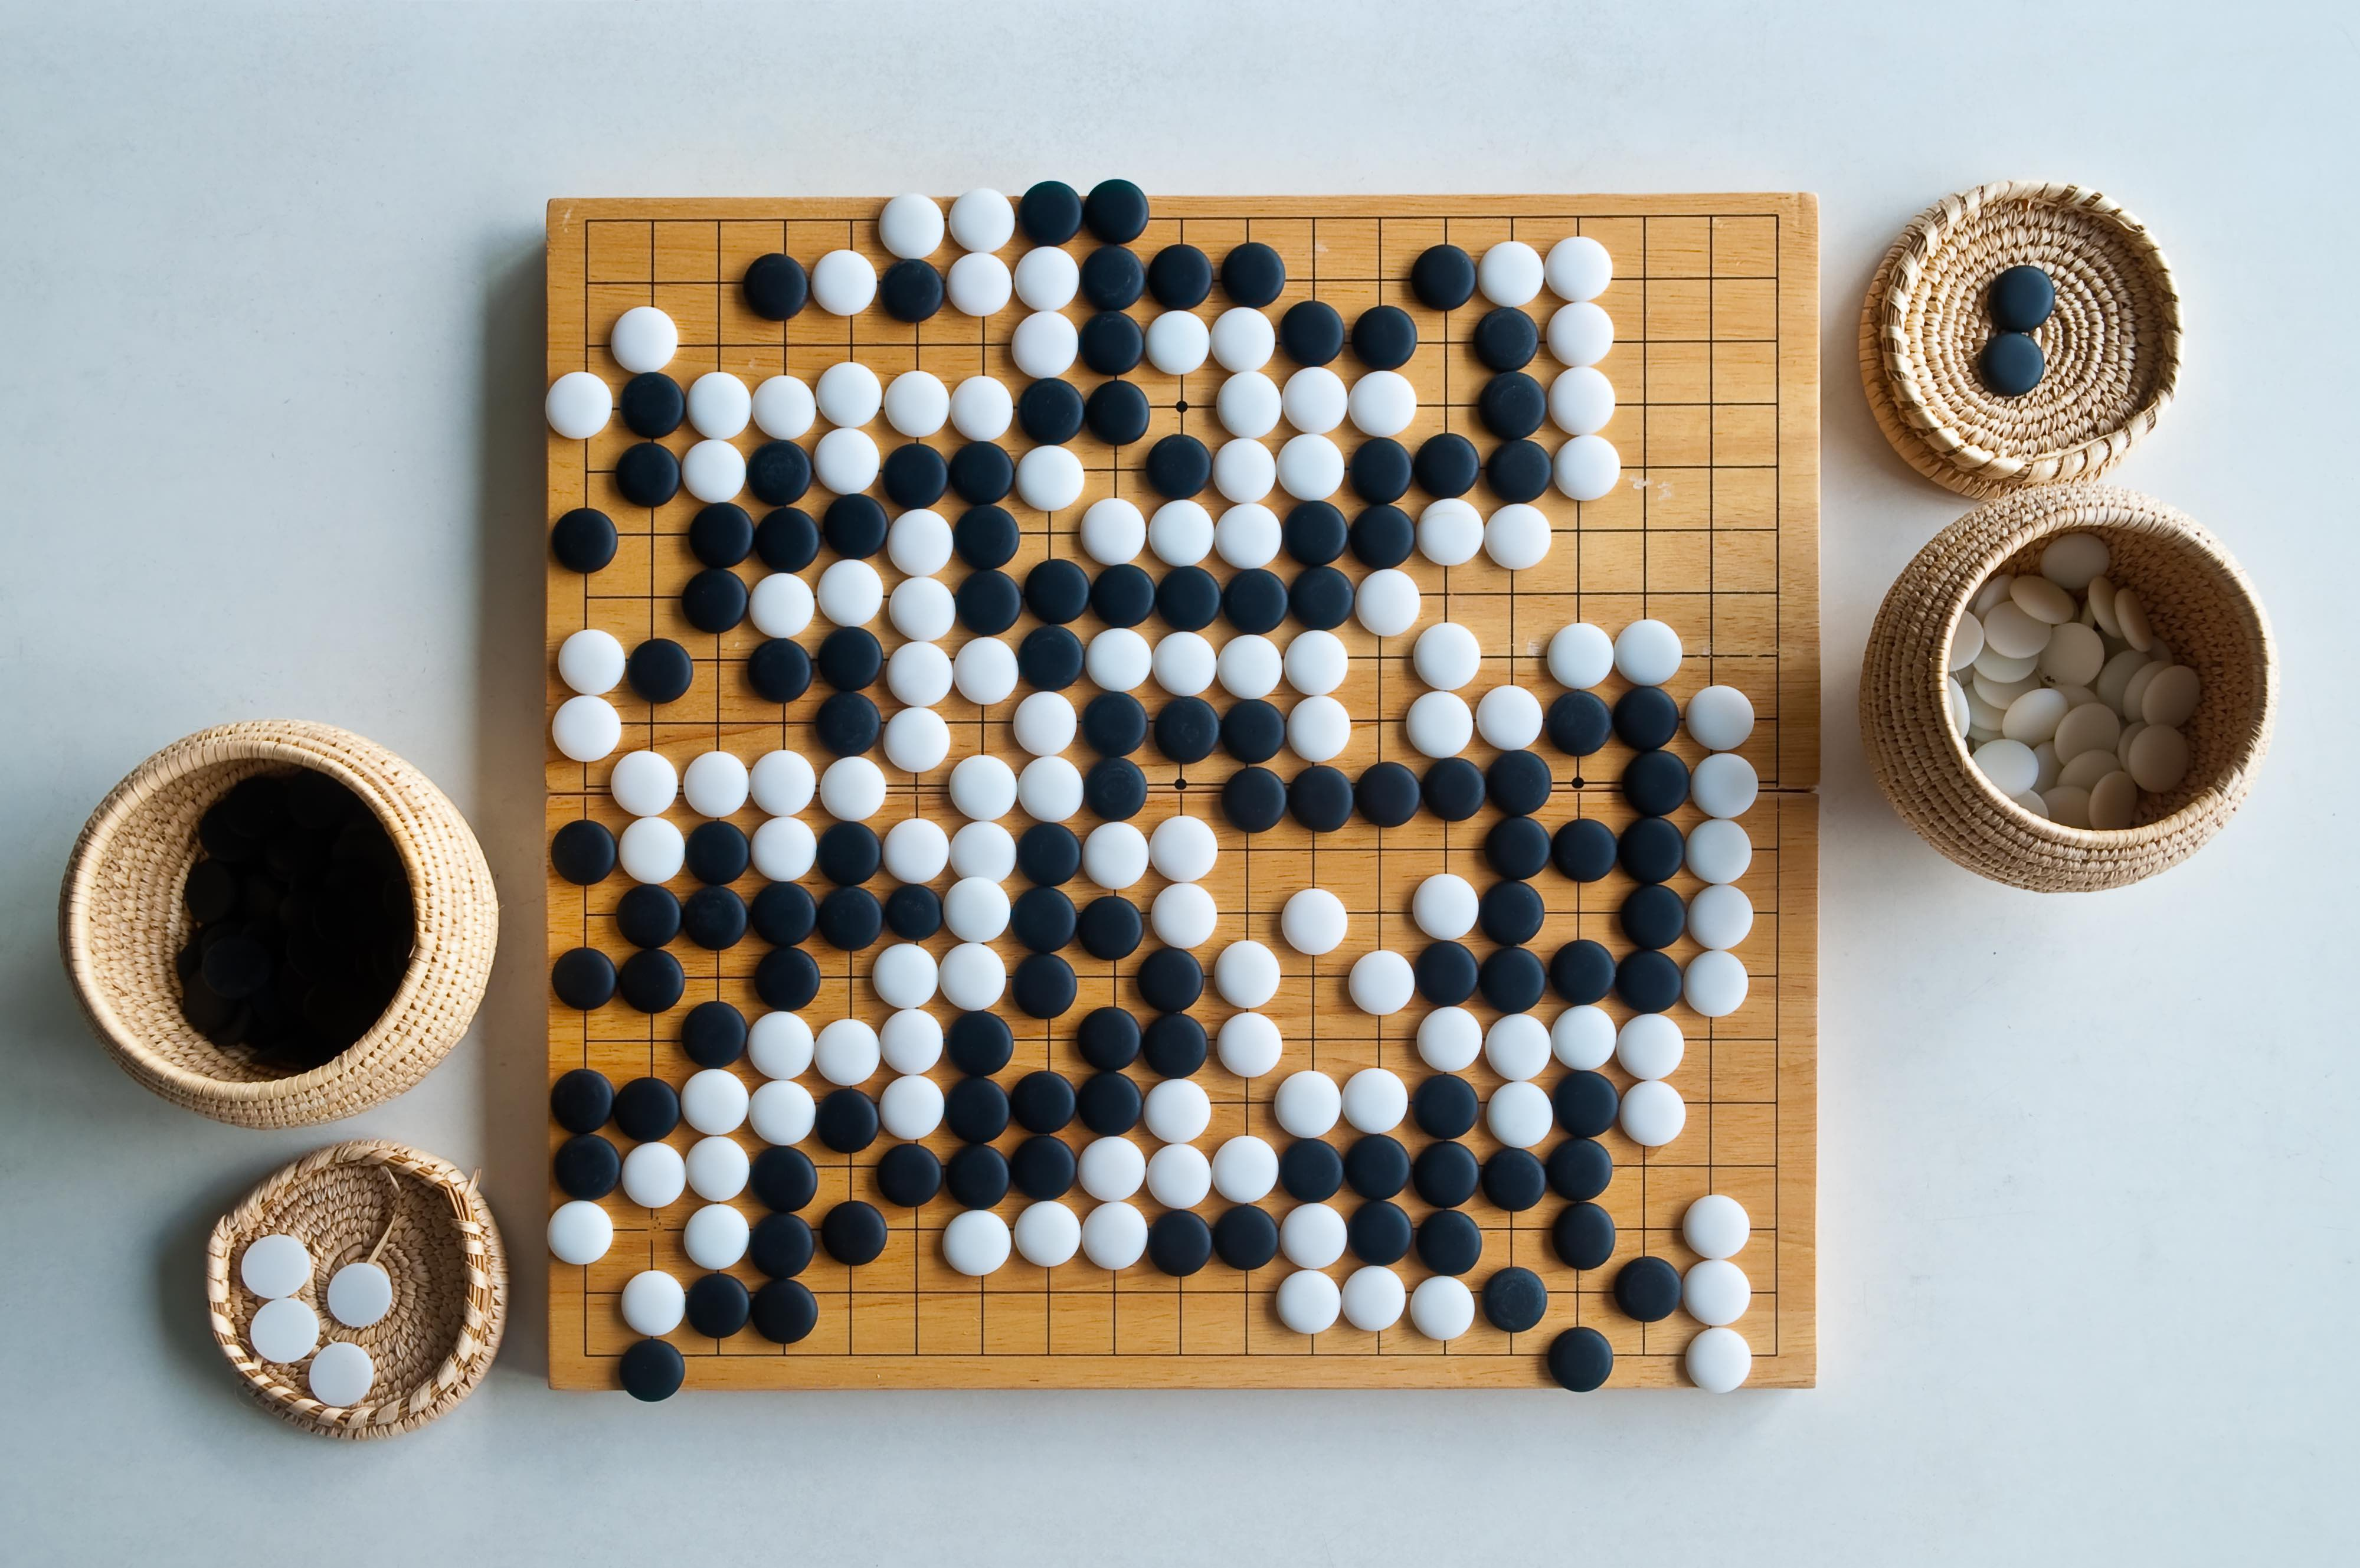
\includegraphics[scale=0.03]{../images/go.jpg}}
      \centering{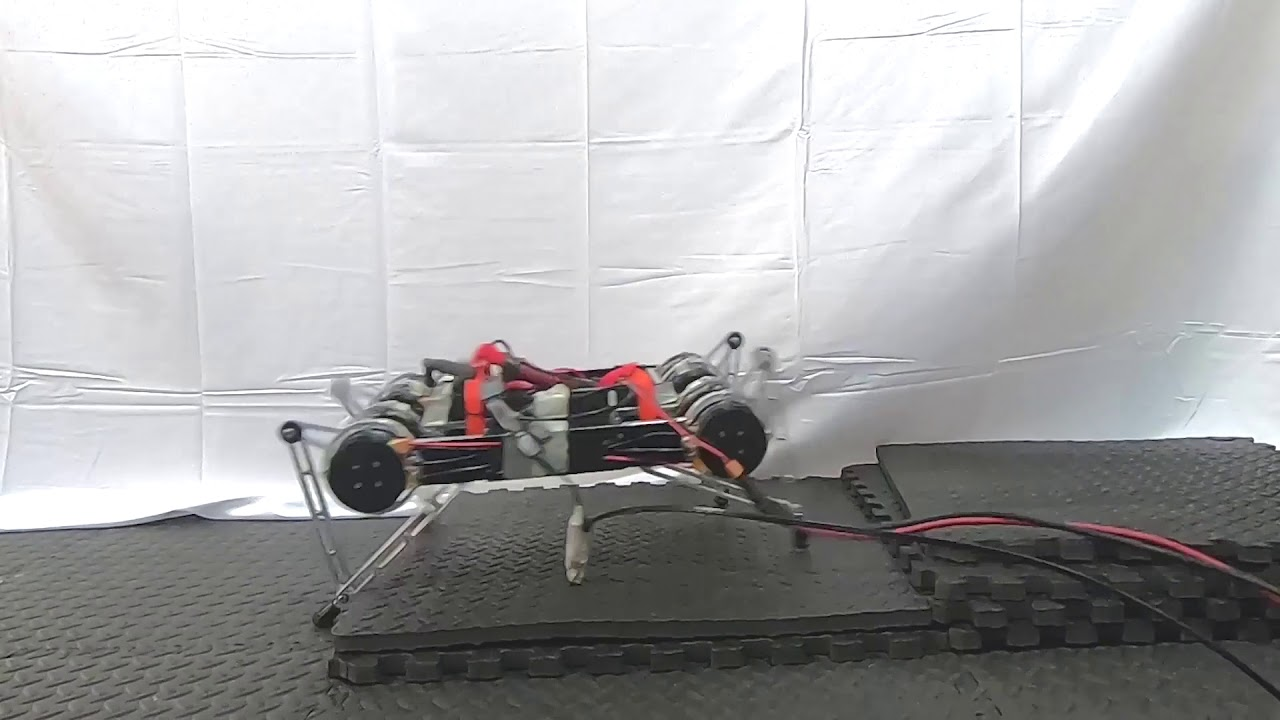
\includegraphics[scale=0.1]{../images/sac_minitaur.jpg}}
    \end{column}


  \end{columns}

\end{frame}


\begin{frame}{\bf reinforcement learning}

  \begin{columns}

    \begin{column}{0.5\textwidth}
      \centering{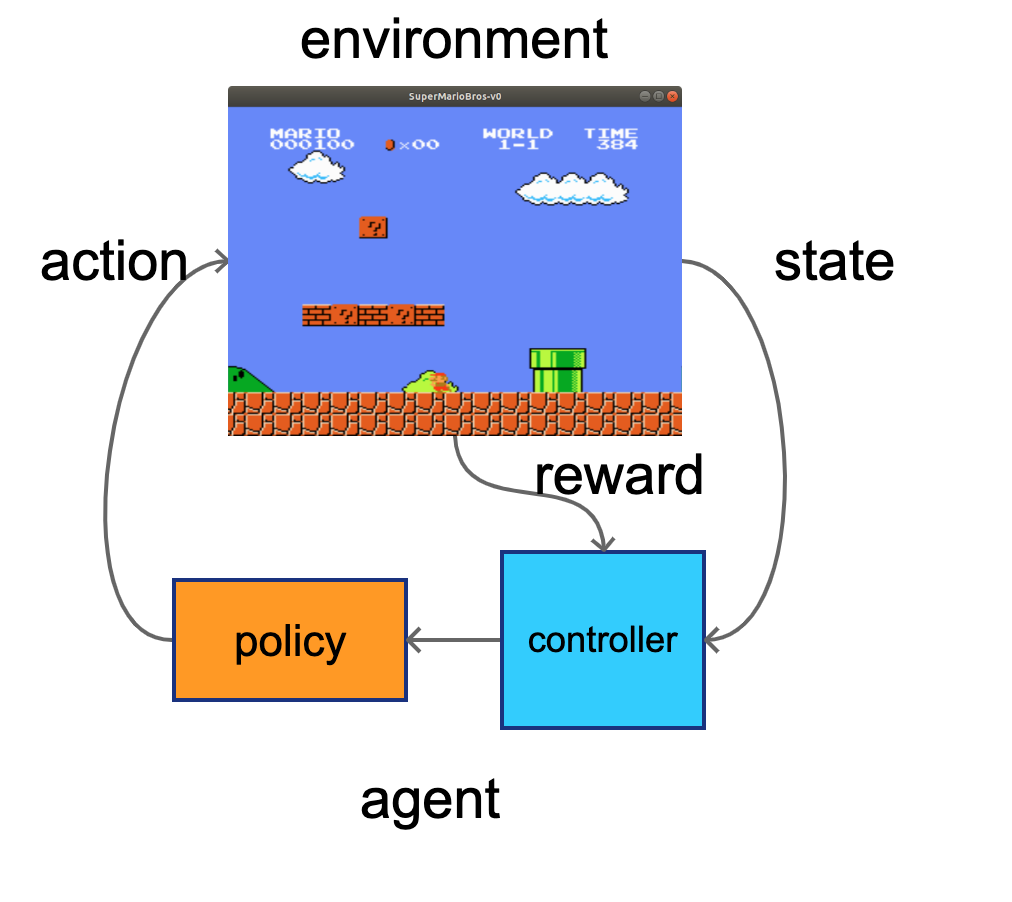
\includegraphics[scale=0.15]{../diagrams/basic/reinforcementlearning.png}}
    \end{column}

    \begin{column}{0.5\textwidth}
      \begin{itemize}
        \item obtain state
        \item select action
        \item exectute action
        \item learn from experiences
      \end{itemize}
    \end{column}

  \end{columns}

\end{frame}


\begin{frame}{\bf action space}

  \begin{itemize}
    \item discrete action space \\
      - keys, keypad
    \item continuous action space \\
      - motors, PWMs, steering, force controll
  \end{itemize}

  \centering{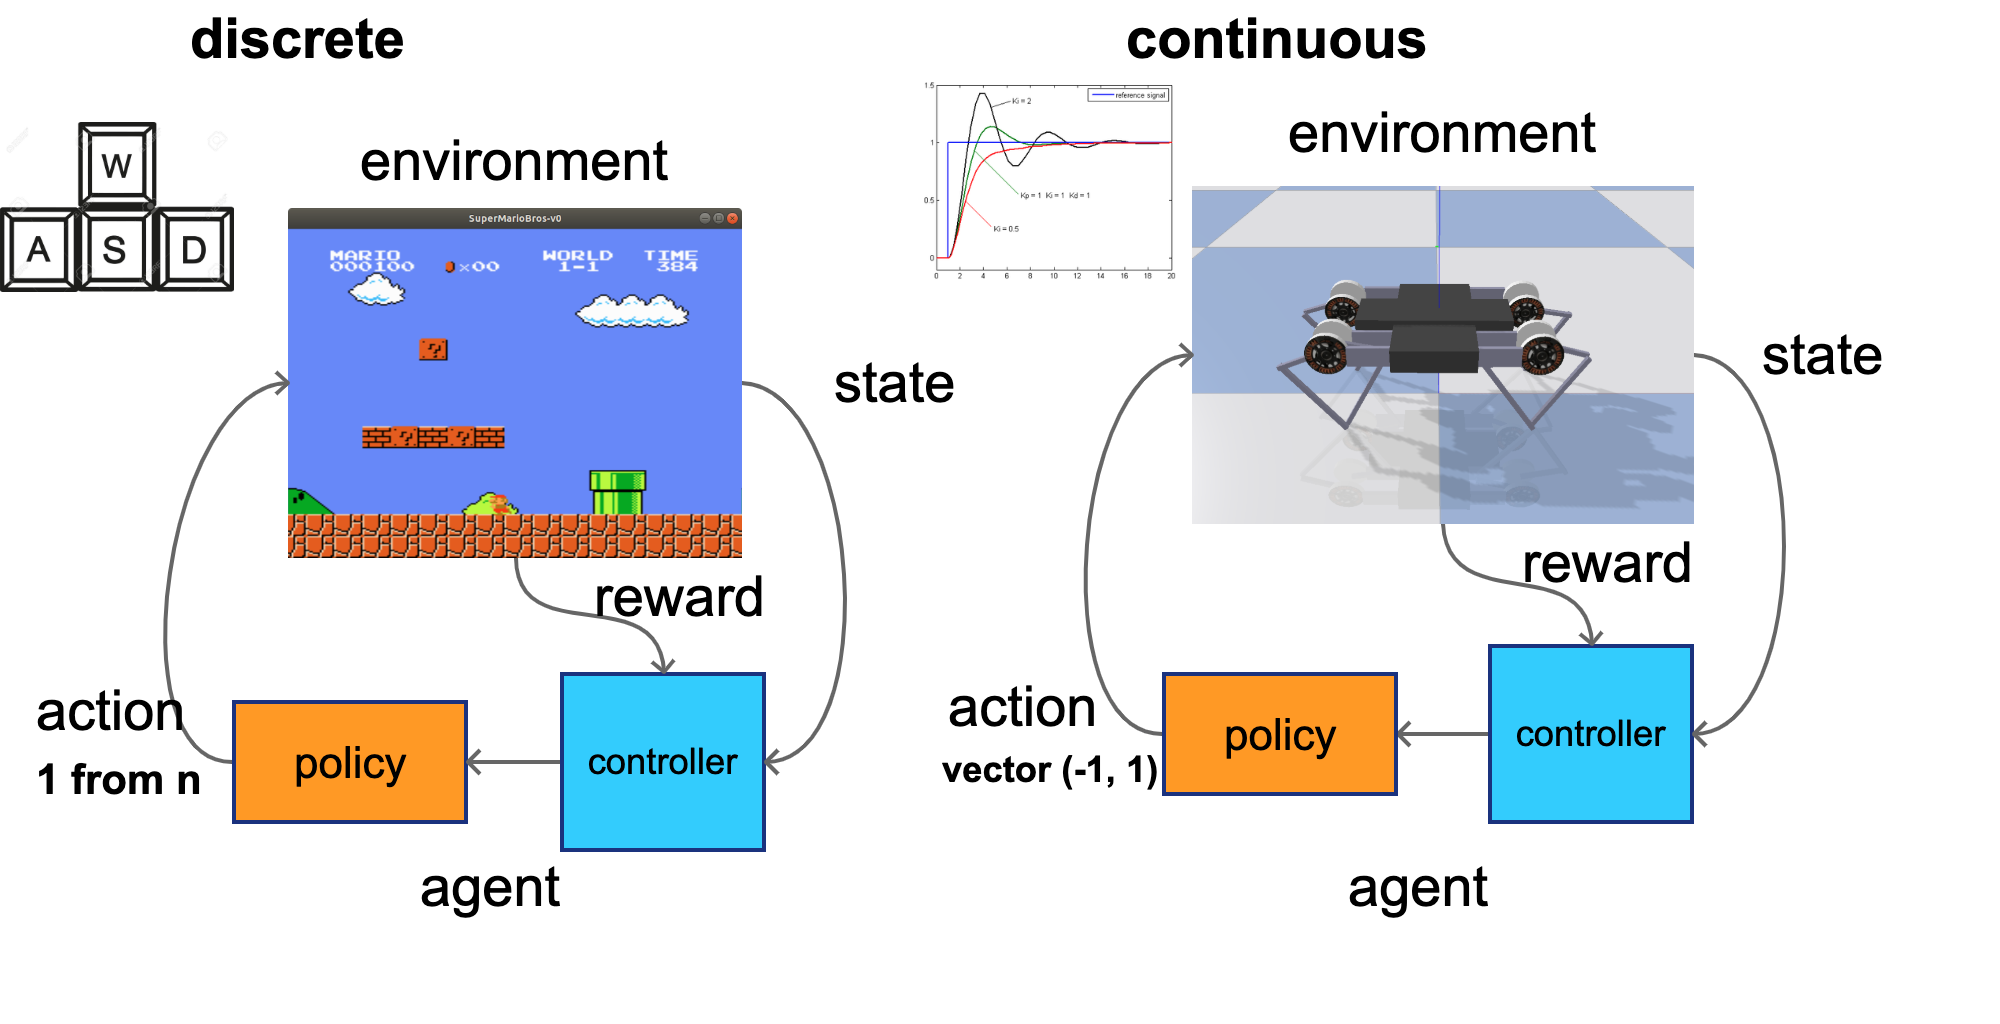
\includegraphics[scale=0.15]{../diagrams/basic/actionspace.png}}

\end{frame}



\begin{frame}{\bf deep Q learning}

  \centering{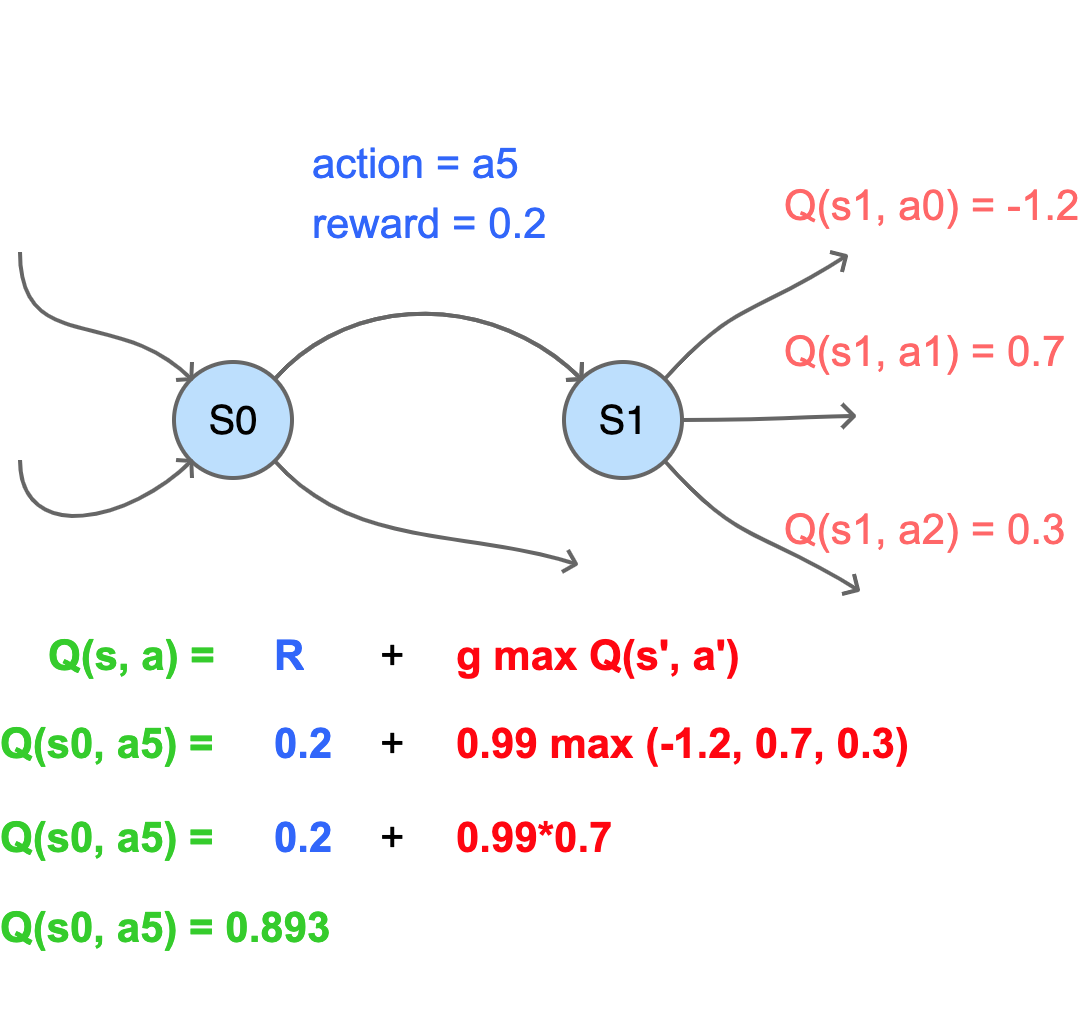
\includegraphics[scale=0.12]{../diagrams/basic/qlearning.png}}

  \begin{align*}
    Q(s, a; \theta) = \underset{\textcolor{cyan}{reward}}{R} + \underset{\textcolor{OrangeRed}{discounted\ future\ reward}}{\gamma \max \limits_{a'} Q(s', a'; \theta^-)}
  \end{align*}

  \begin{align*}
    \mathcal{L(\theta)} = \left( R + \gamma \max \limits_{a'} Q(s', a'; \theta^-) - Q(s, a; \theta)  \right)^2
  \end{align*}
\end{frame}

\begin{frame}{\bf deep Q learning}

  \centering{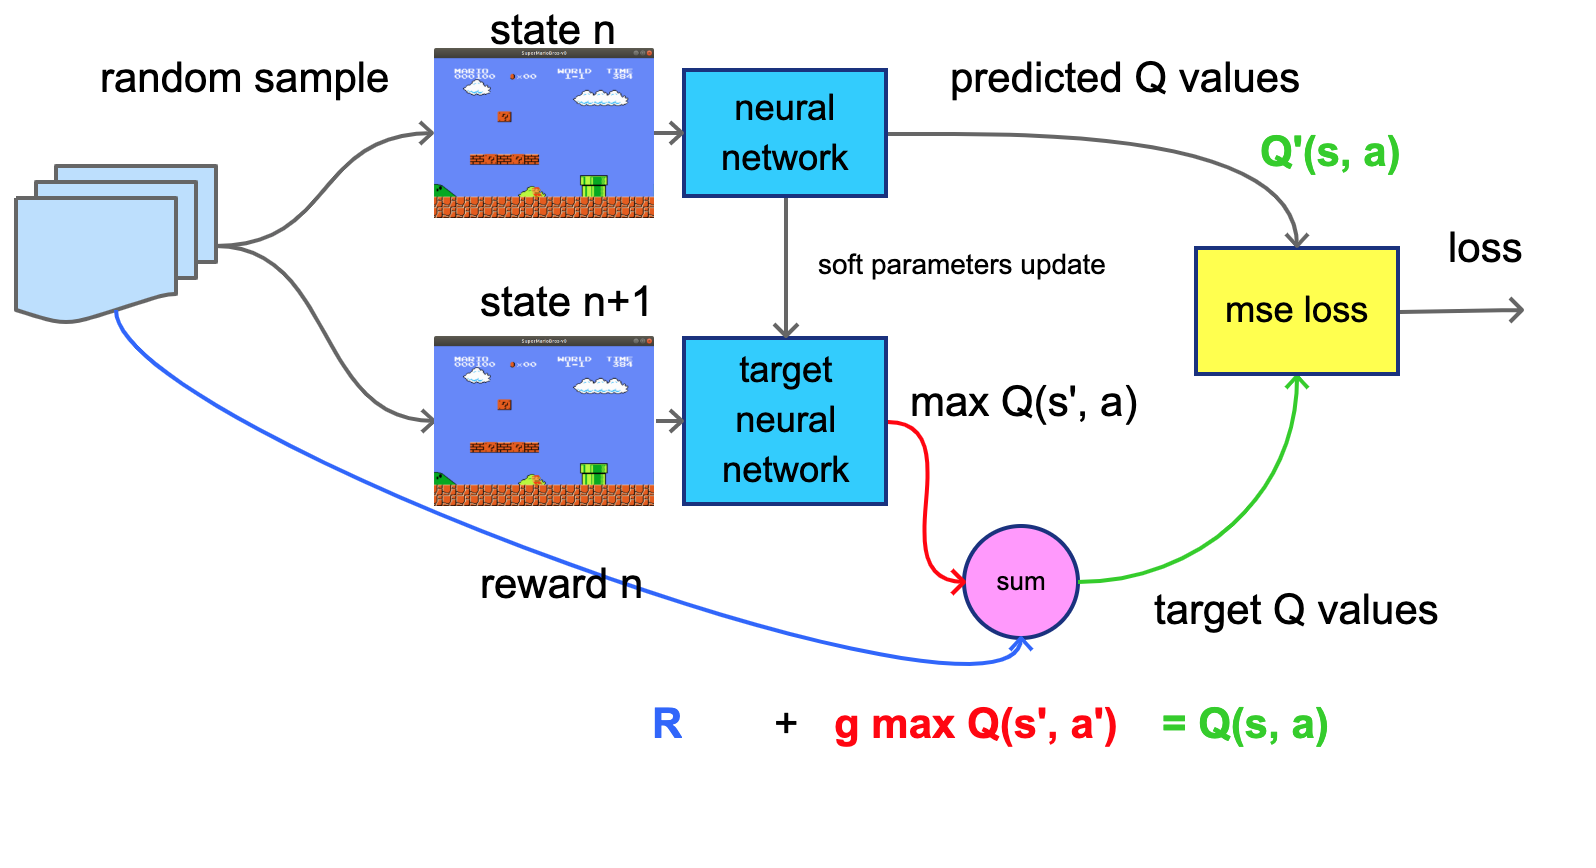
\includegraphics[scale=0.15]{../diagrams/basic/deepqlearningdetail.png}}

  \begin{align*}
    Q(s, a; \theta) = \underset{\textcolor{cyan}{reward}}{R} + \underset{\textcolor{OrangeRed}{discounted\ future\ reward}}{\gamma \max \limits_{a'} Q(s', a'; \theta^-)}
  \end{align*}

  \begin{align*}
    \mathcal{L(\theta)} = \left( R + \gamma \max \limits_{a'} Q(s', a'; \theta^-) - Q(s, a; \theta)  \right)^2
  \end{align*}
\end{frame}




\begin{frame}{\bf deep deterministic policy gradietnt}

  {\bf DDPG}

  \begin{itemize}
    \item continuous action space
    \item natural extension of DQN
    \item actor-critic structure
  \end{itemize}

  \centering{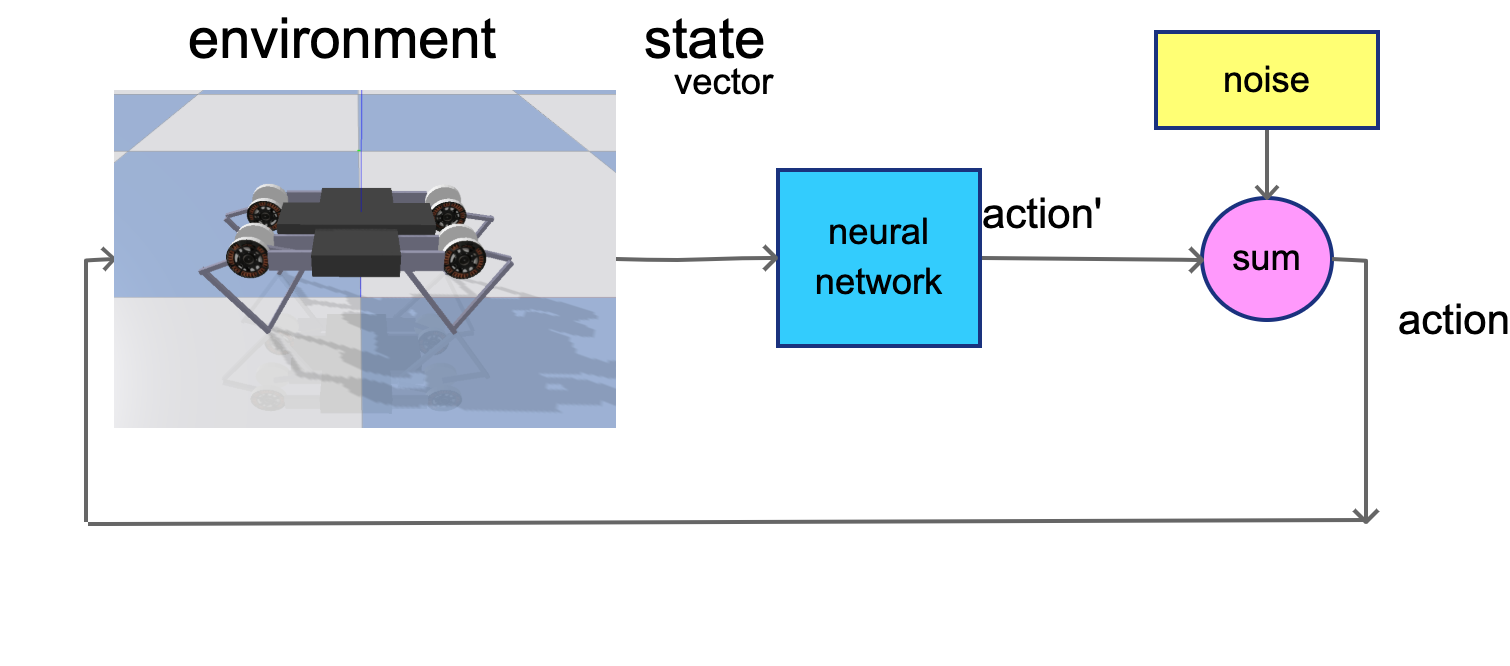
\includegraphics[scale=0.15]{../diagrams/basic/ddpgnetwork.png}}

\end{frame}




\begin{frame}{\bf DDPG}

  \centering{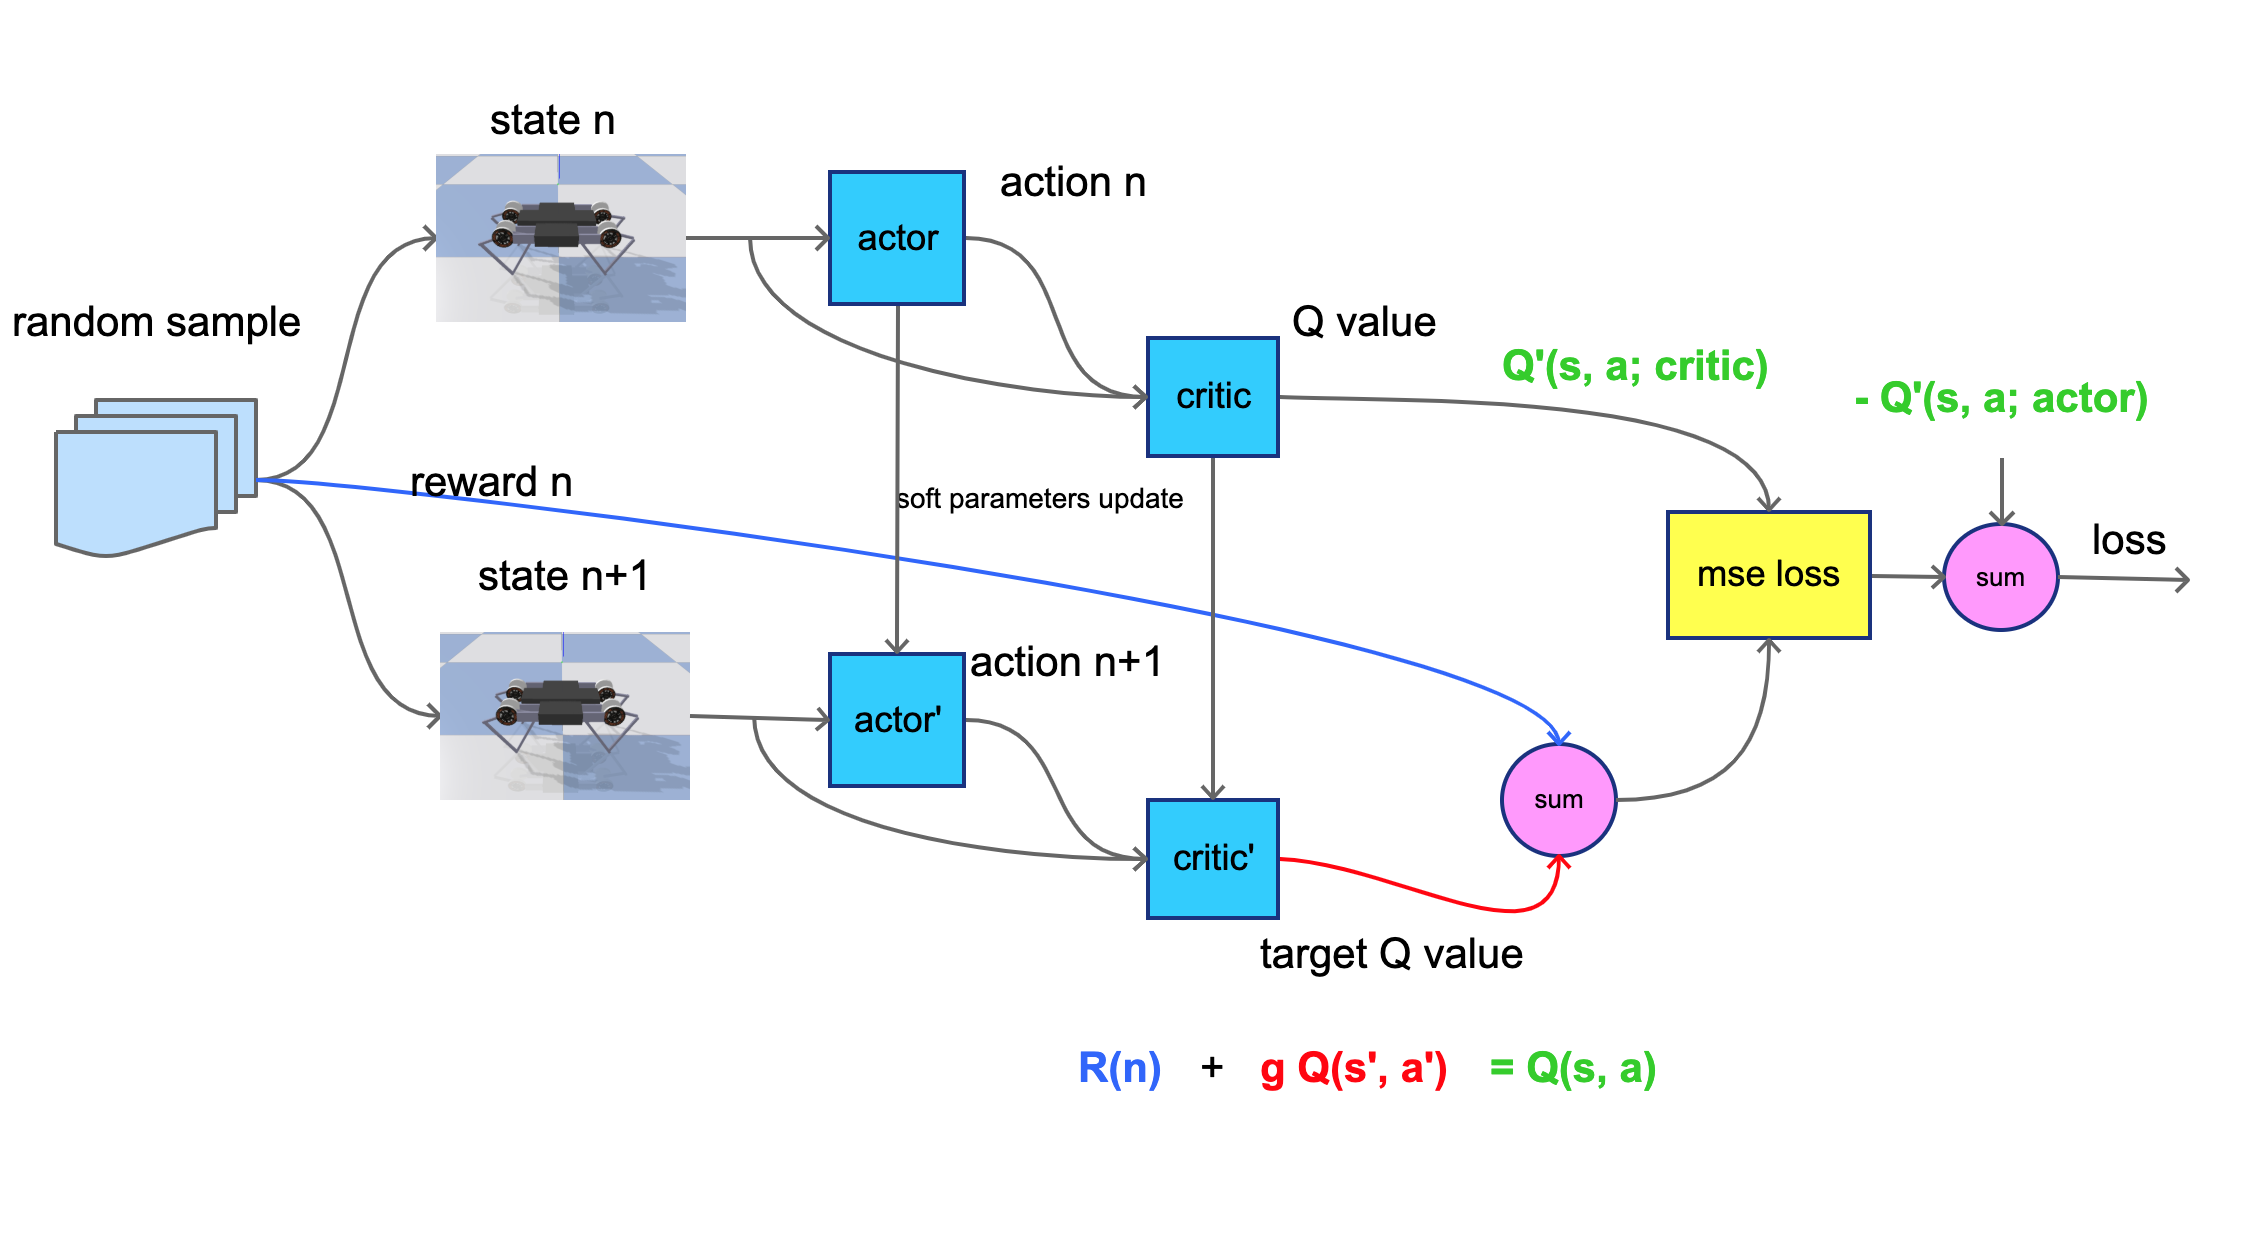
\includegraphics[scale=0.12]{../diagrams/basic/ddpgtraining.png}}

\end{frame}


\begin{frame}{\bf DDPG}

  \centering{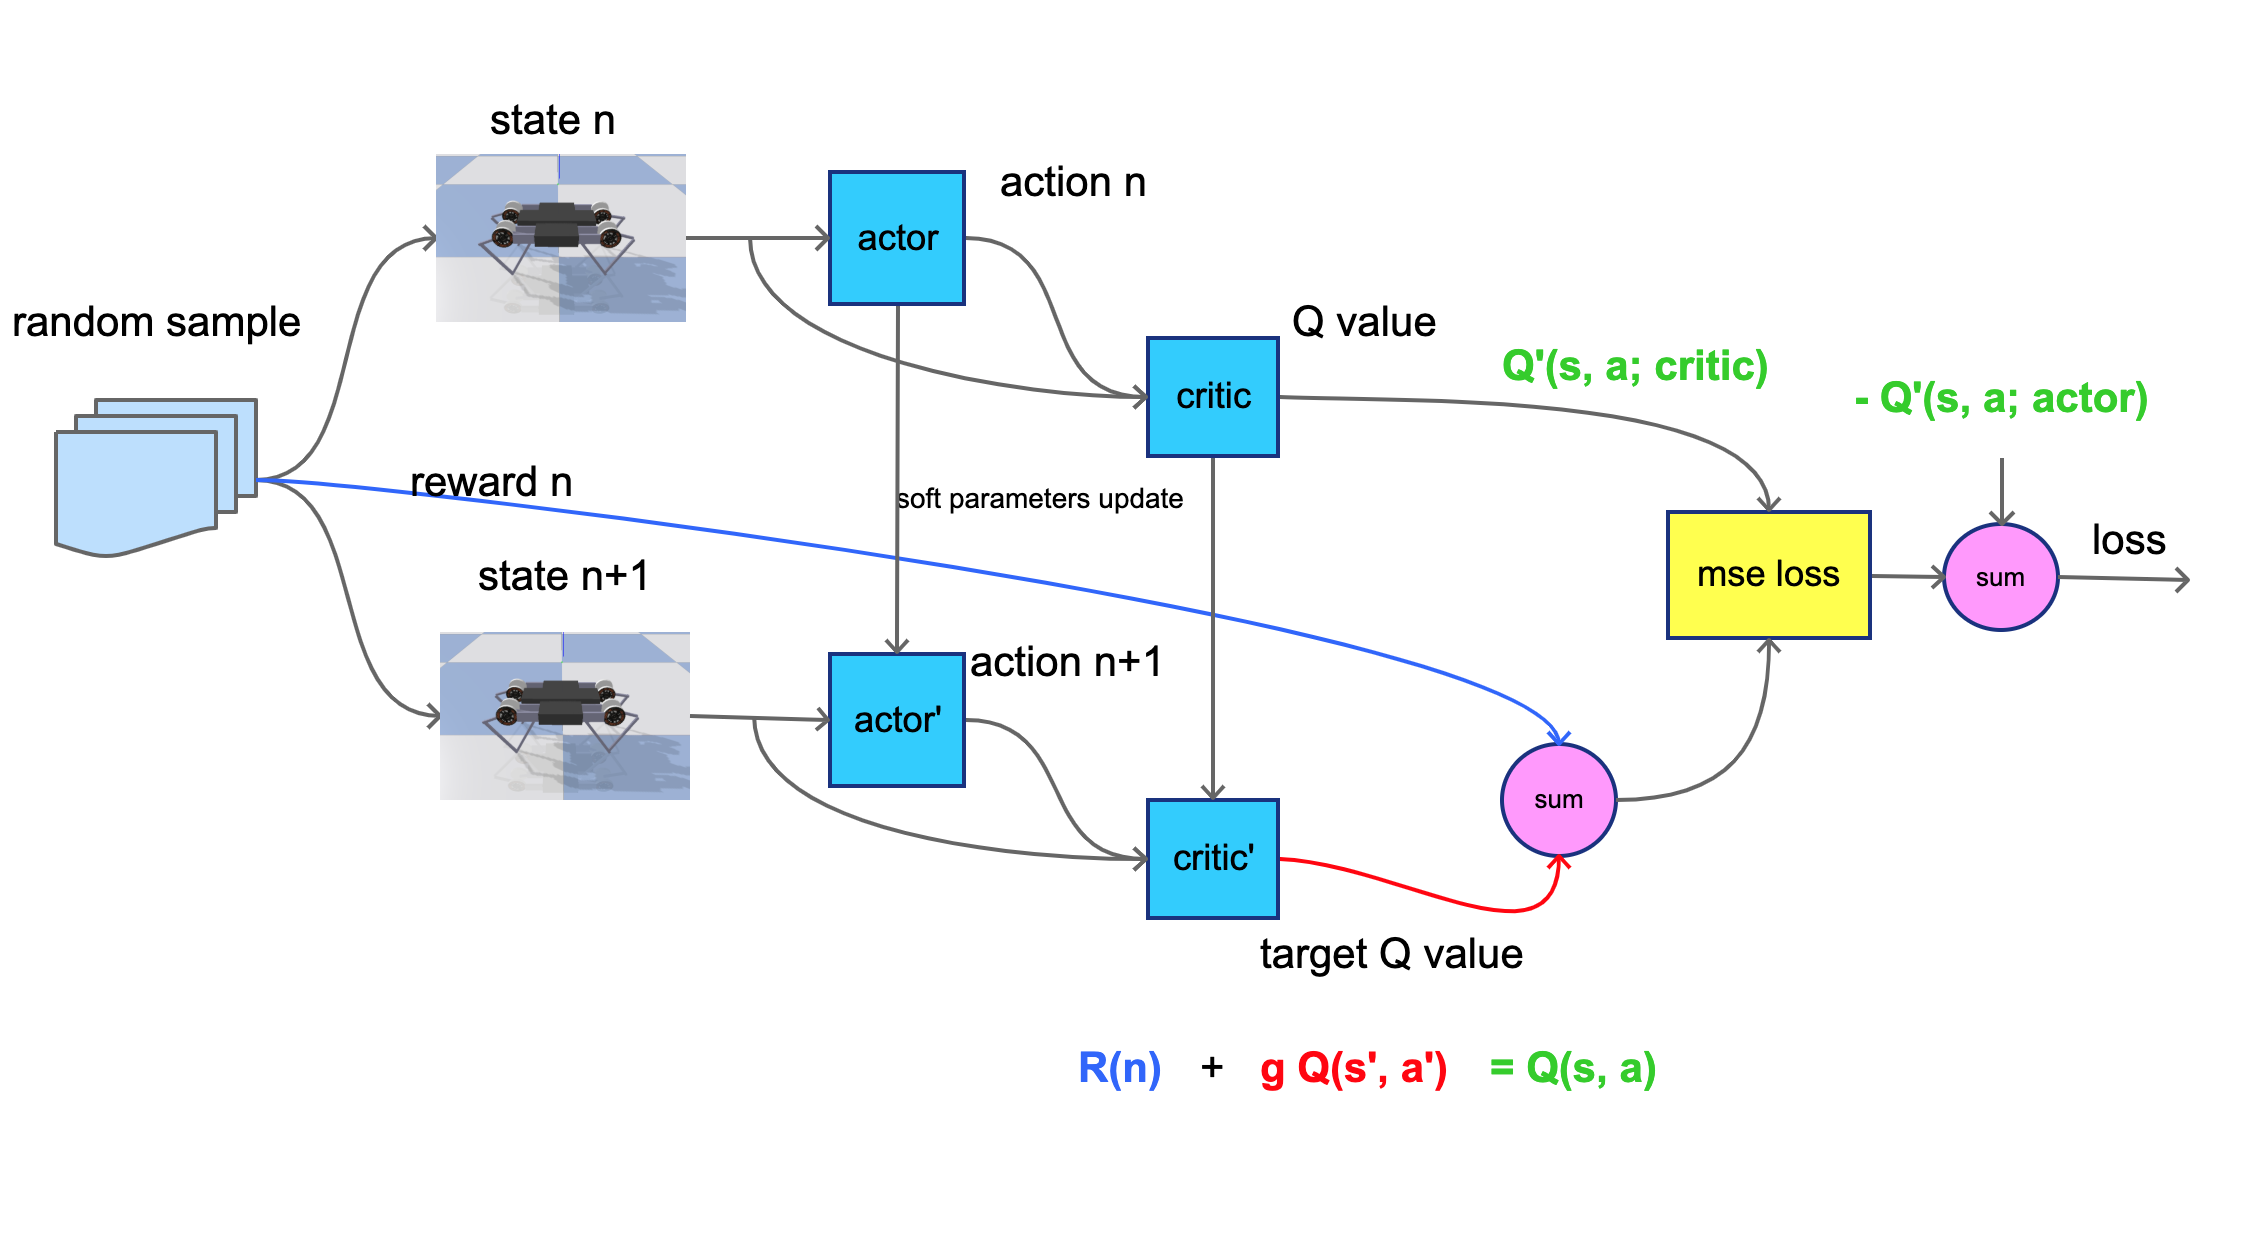
\includegraphics[scale=0.08]{../diagrams/basic/ddpgtraining.png}}

  \begin{align*}
    \mathcal{L(\theta)} &= \left( R + \gamma Q(s', A(s'; \phi^-); \theta^-) - Q(s, A(s; \phi); \theta)  \right)^2 \\
    \mathcal{L(\phi)} &= -Q(s, A(s; \phi); \theta)
  \end{align*}

  where
  \begin{itemize}
    \item $Q$ is critic network with parameters $\theta$
    \item $A$ is actor network with parameters $\phi$
  \end{itemize}
  
\end{frame}



\begin{frame}{\bf wise Wizard's DDPG spell chart}
  \begin{itemize}
    \item {\bf \color{red} neurons count} on 1st layer = 10x  state vector size
    \item {\bf \color{red} neurons count} on 2nd layer = 0.5x neurons on 1st layer
    \item {\bf \color{red} weight init} for hidden layers : use Xavier
    \item {\bf \color{red} weight init} actor output  : use uniform $\langle -0.3, 0.3 \rangle$
    \item {\bf \color{red} weight init} critic output : use uniform $\langle -0.003, 0.003 \rangle$
    \item {\bf \color{red} gaussian noise} : linear decay variance, from 0.5 to 0.1, for 1M steps, or noisy layers
    \item use {\bf \color{red} soft} target network update, $\tau = 0.001$
    \item actor learning rate $\eta_a = 0.0001$
    \item critic learning rate $\eta_c = 0.0002$
  \end{itemize}
\end{frame}


\begin{frame}{\bf wise Wizard's magic staff}

  \begin{columns}

    \begin{column}{0.5\textwidth}
      \begin{itemize}
        \item fully connected nets (robotic envs) {\bf \color{red} train on CPU} - AMD Ryzen
        \item convolutional nets (visual inputs envs) {\bf \color{red} train on GPU}
        \item use fast CPU - envs are slow
        \item 32GB of RAM is enough
        \item for small visual envs (Atari, DOOM, Nec) - GTX1060, GTX1080ti, RTX2080 ...
      \end{itemize}
    \end{column}

    \begin{column}{0.5\textwidth}
      {\centering 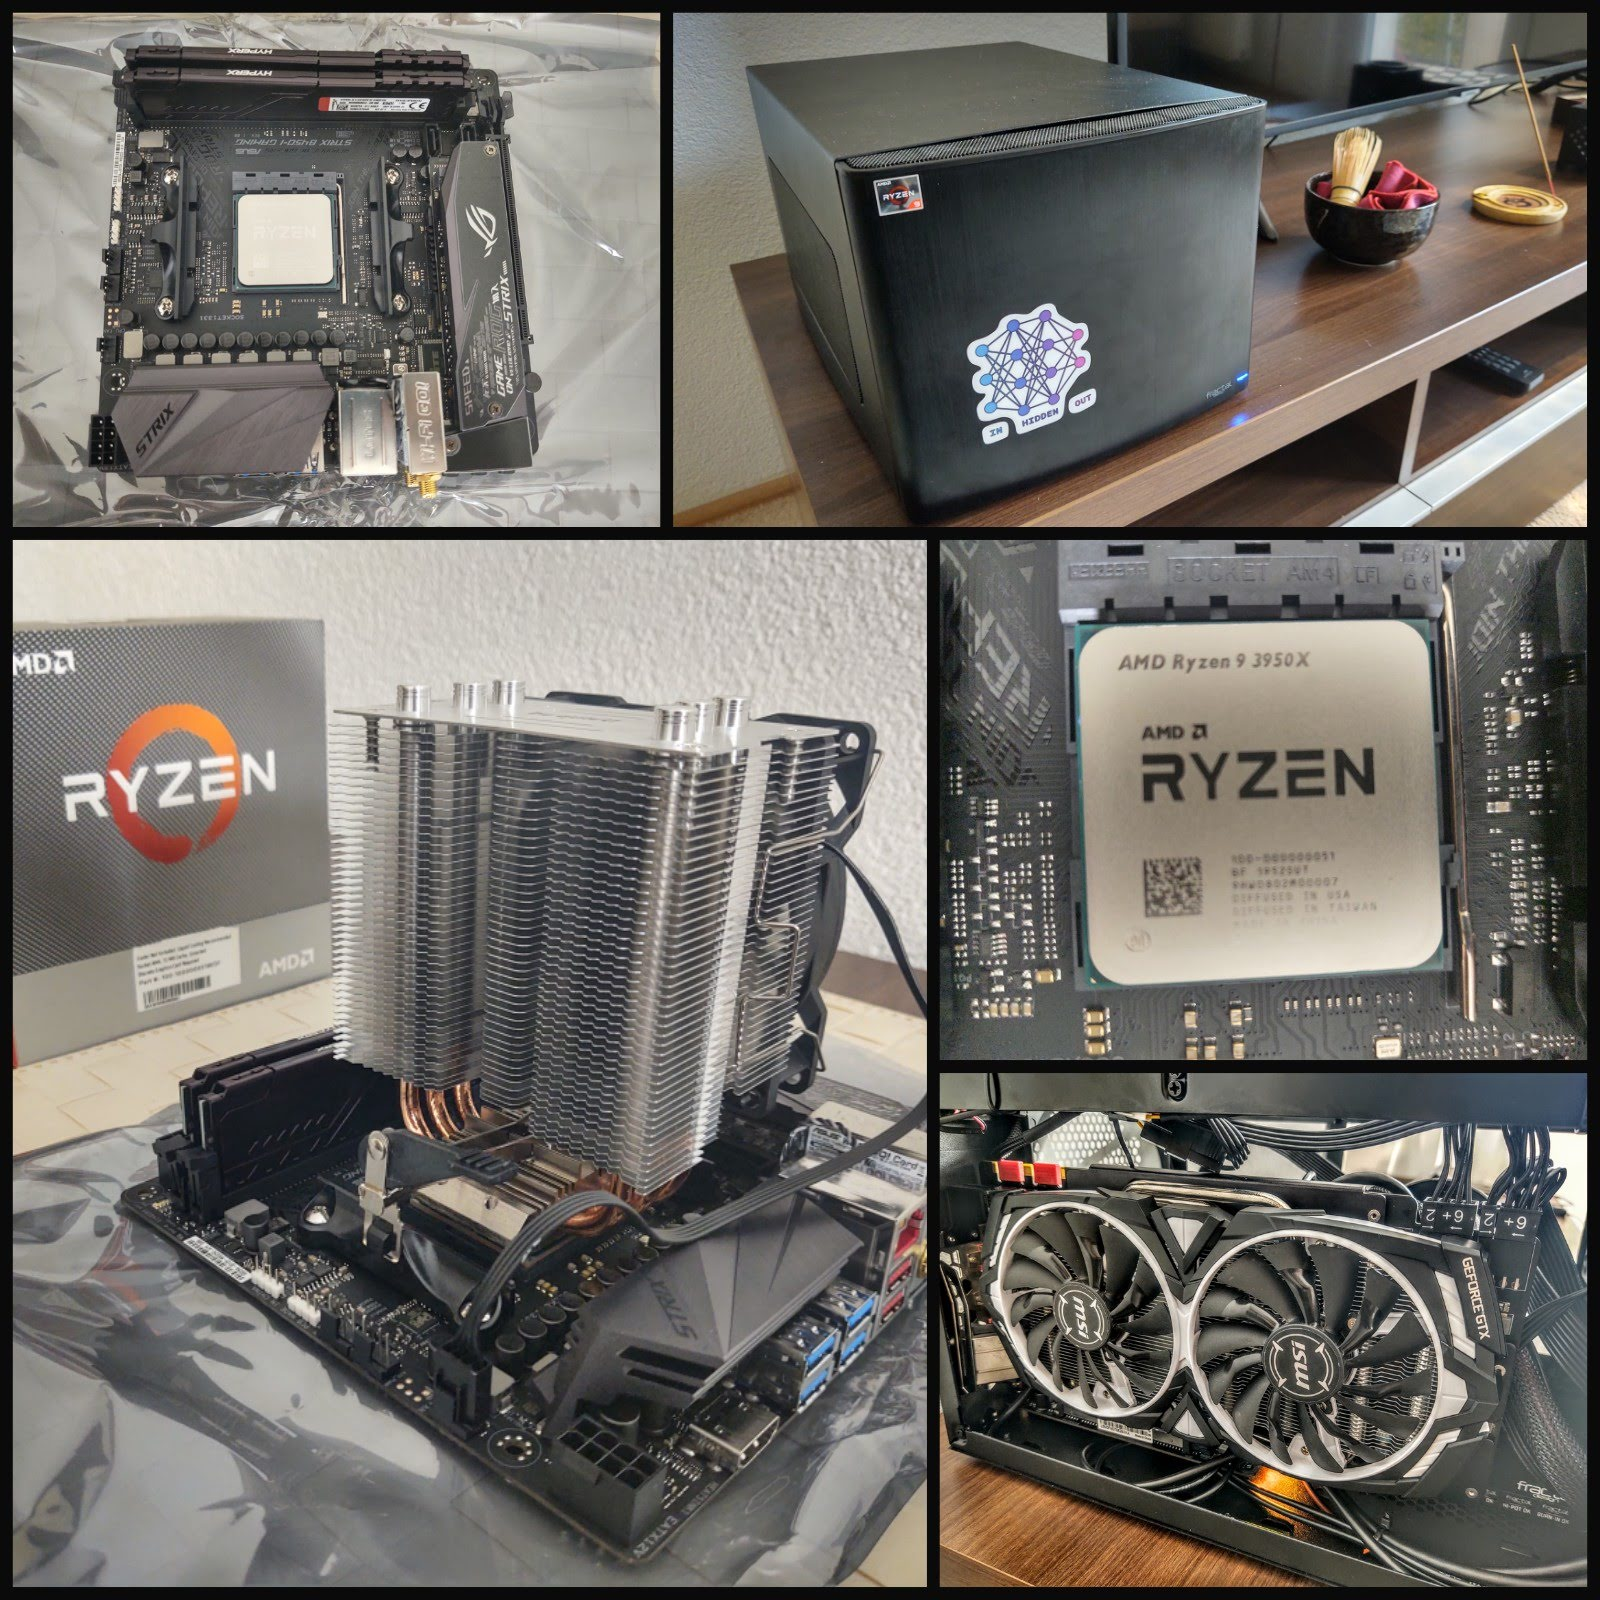
\includegraphics[scale=0.1]{../images/computer.jpg}}
    \end{column}

  \end{columns}


\end{frame}


\begin{frame}{\bf books to read}

        \begin{itemize}
          \item Maxim Lapan, 2020, Deep Reinforcement Learning Hands-On second edition
          \item Maxim Lapan, 2018, Deep Reinforcement Learning Hands-On
          \item Praveen Palanisamy, 2018, Hands-On Intelligent Agents with OpenAI Gym
          \item Andrea Lonza, 2019, Reinforcement Learning Algorithms with Python
          \item Rajalingappaa Shanmugamani, 2019, Python Reinforcement Learning
          \item Micheal Lanham, 2019, Hands-On Deep Learning for Games
        \end{itemize}

\end{frame}


\begin{frame}{\bf Q\&A}

\centering{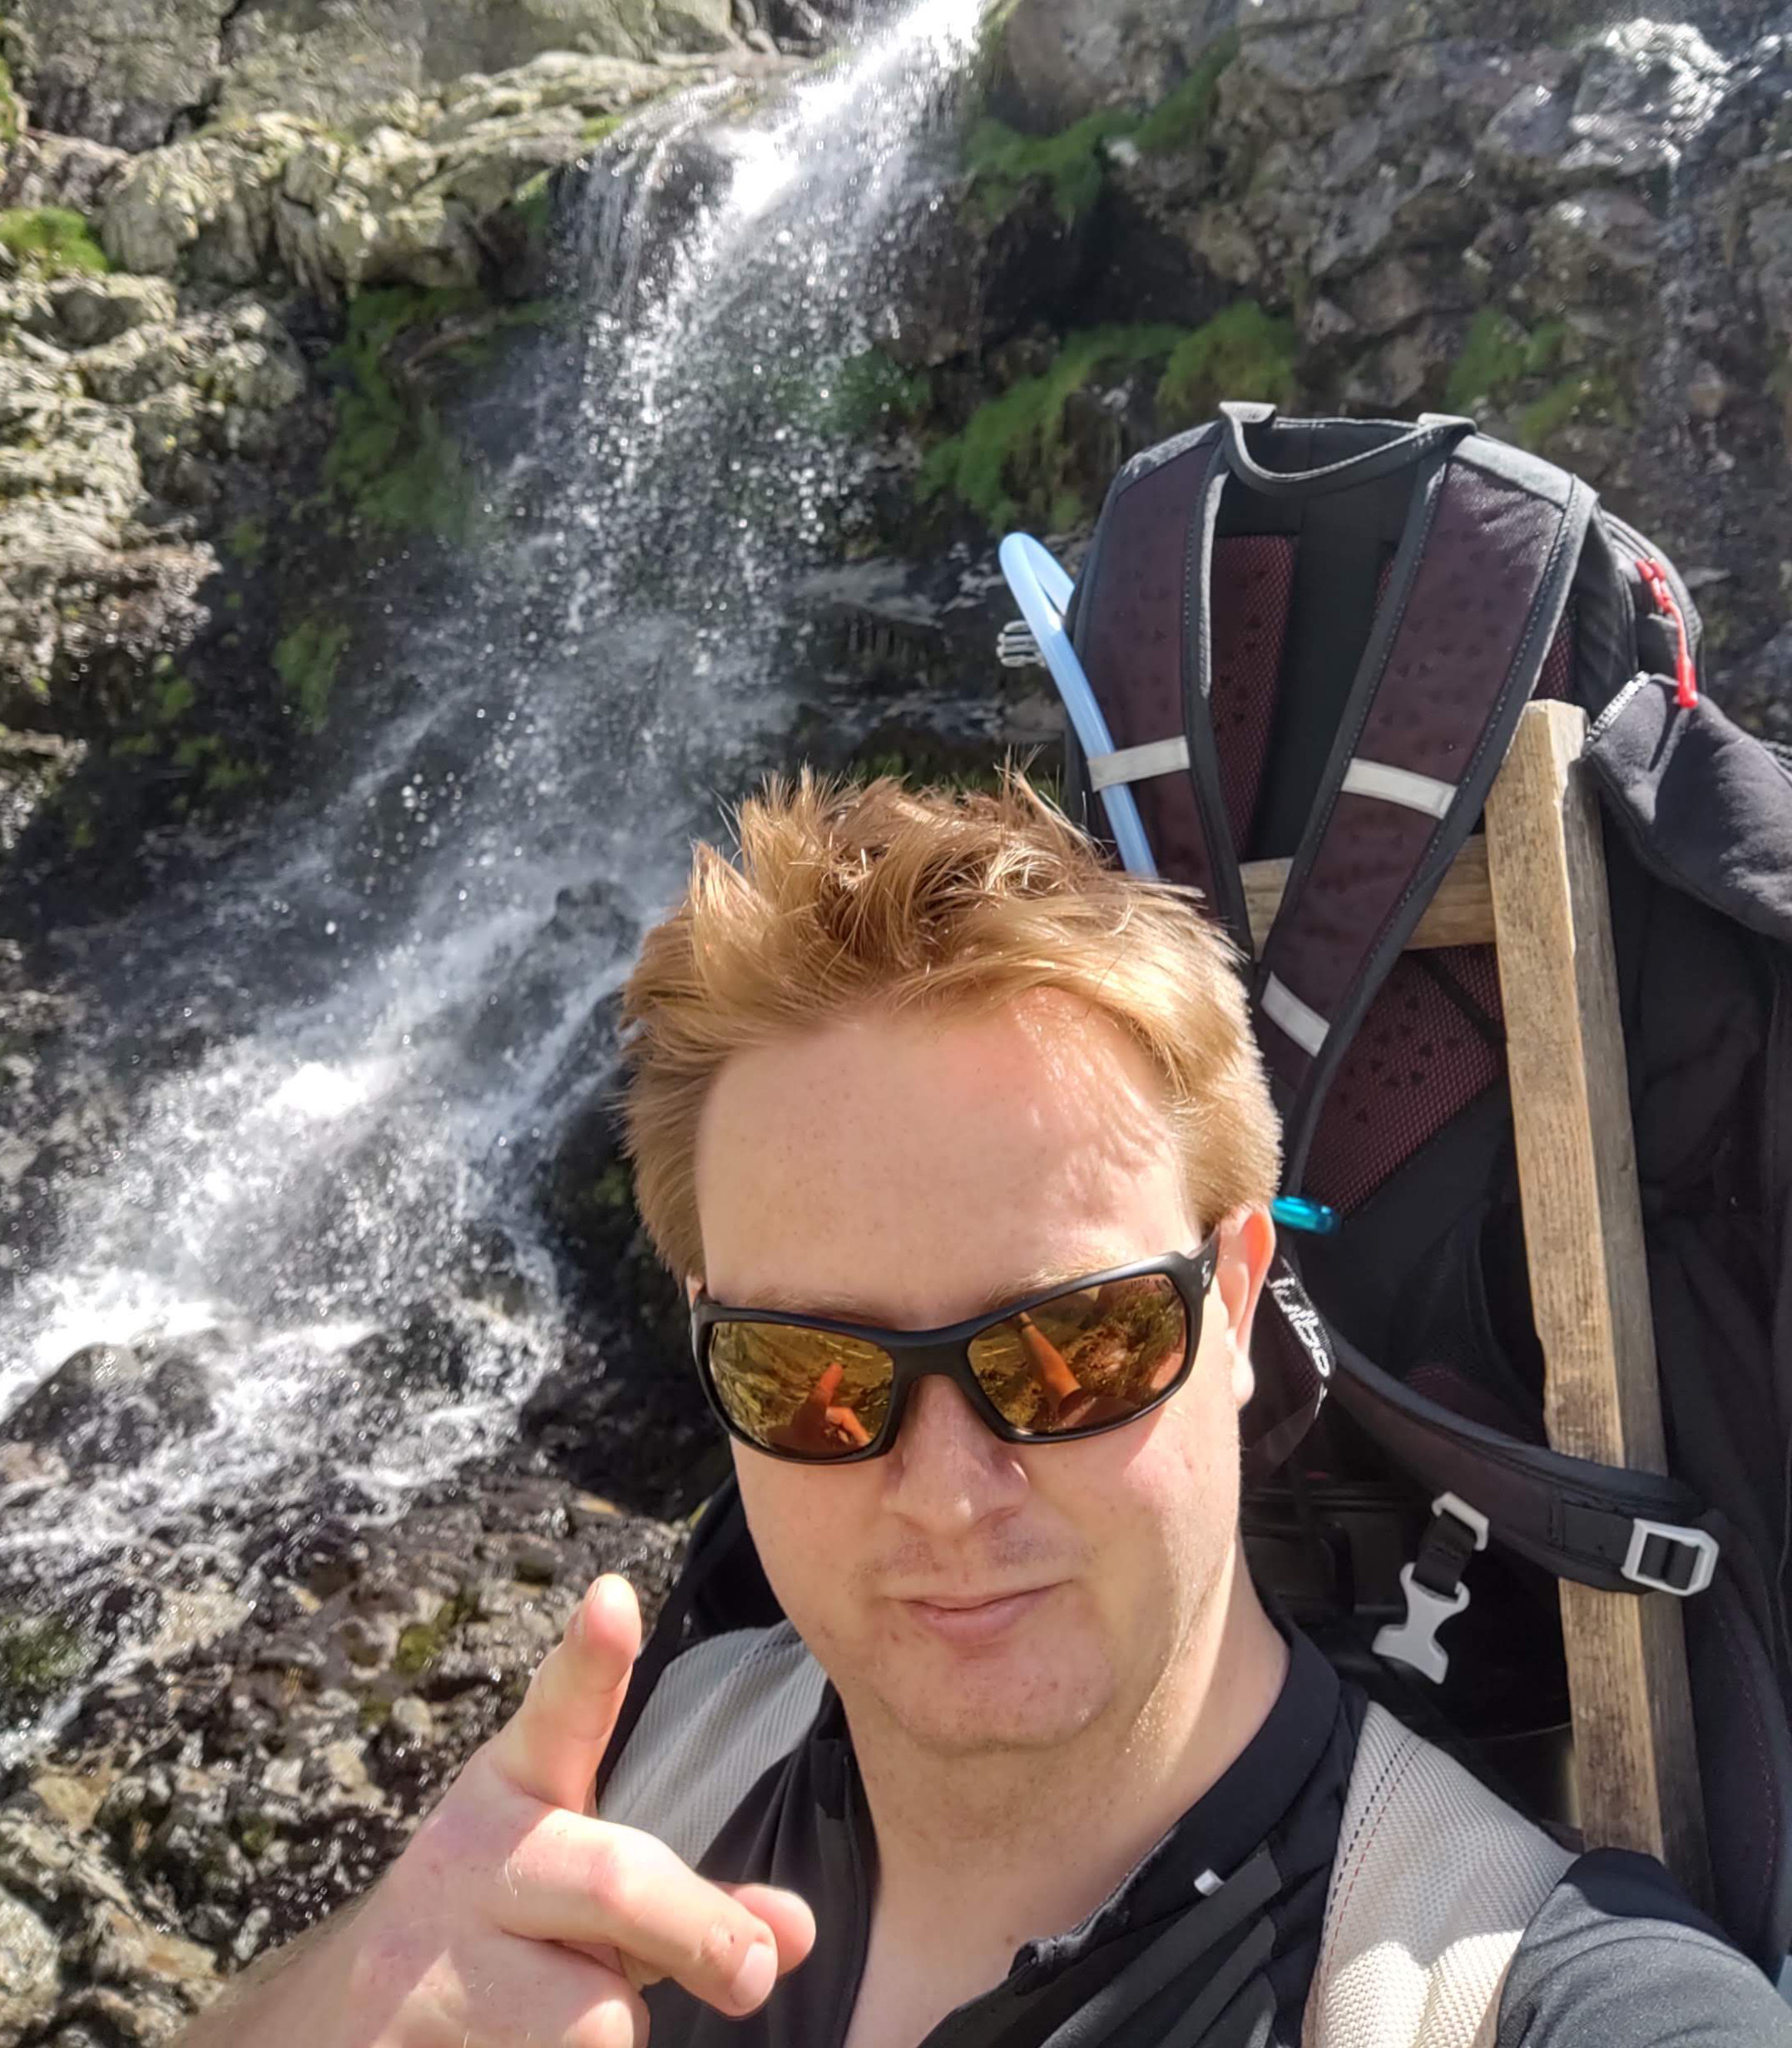
\includegraphics[scale=0.1]{../images/me.jpg}}

\url{michal.nand@gmail.com}

\url{https://github.com/michalnand/reinforcement_learning_tutorial}

 
\end{frame}


\end{document}
